\begin{frame}{Le stockage dans SAVOIE}
\begin{block}{Principes}
\begin{itemize}
    \item Le stockage de SAVOIE repose sur deux SAN
    \item Clusterisation des SAN en mode maître-esclave
    \item Vu de l'extérieur, c'est comme si on n'avait qu'un seul SAN maître portant la @vIP
\end{itemize}
\end{block}
\end{frame}

\begin{frame}{Avantages et inconvénients d'un SAN}
\begin{block}{Avantages}
\begin{itemize}
    \item Avantage d'un stockage distant sur un stockage local
    \item Meilleure évolutivité
    \item Faire reposer une partie de la charge CPU sur les SAN \pause
\end{itemize}
\end{block}
\begin{block}{Inconvénients}
\begin{itemize}
          \item Forte dépendance au SAN
          \item Forte dépendance au réseau reliant le SAN aux ESX (VLAN STOCKAGE) en termes de performances et de disponibilité
\end{itemize}
\end{block}
\end{frame}

\begin{frame}{RAID 10}
\begin{block}{Fonctionnement}
\begin{itemize}
\item 2 disques en RAID0 : répartir les informations stockées sur plusieurs disques durs grâce à un entrelacement des données. Temps d'accès accéléré.
\item 2 disques en RAID1 : l’un est utilisé en miroir de l'autre
\end{itemize}
\end{block}
\begin{block}{Avantages et inconvénients}
\begin{itemize}
\item Permet la performance et la disponibilité
\item Performance de 50\% (4*6To=>12To)
\end{itemize}
\end{block}
\end{frame}

\begin{frame}{Comment le stockage est-il réalisé dans SAVOIE ?}
\begin{center}
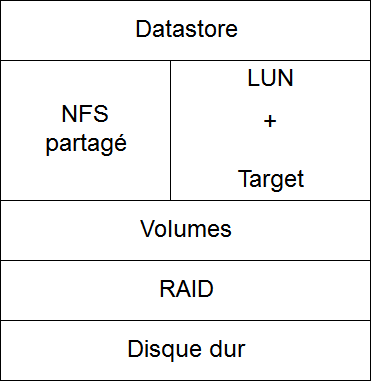
\includegraphics[width=200px]{Schemas/Concepts_Stockage.png}
\end{center}
\end{frame}
